\documentclass[a4paper,14pt]{article}
\usepackage{float}
\usepackage{extsizes}
\usepackage{amsmath}
\usepackage{amssymb}
\everymath{\displaystyle}
\usepackage{geometry}
\usepackage{fancyhdr}
\usepackage{multicol}
\usepackage{graphicx}
\usepackage[brazil]{babel}
\usepackage[shortlabels]{enumitem}
\usepackage{cancel}
\usepackage{textcomp}
\usepackage{array} % Para melhor formatação de tabelas
\usepackage{longtable}
\usepackage{booktabs}  % Para linhas horizontais mais bonitas
\usepackage{float}   % Para usar o modificador [H]
\usepackage{caption} % Para usar legendas em tabelas
\usepackage{tcolorbox}

\columnsep=2cm
\hoffset=0cm
\textwidth=8cm
\setlength{\columnseprule}{.1pt}
\setlength{\columnsep}{2cm}
\renewcommand{\headrulewidth}{0pt}
\geometry{top=1in, bottom=1in, left=0.7in, right=0.5in}

\pagestyle{fancy}
\fancyhf{}
\fancyfoot[C]{\thepage}

\begin{document}
	
	\noindent\textbf{6FMA57 - Matemática} 
	
	\begin{center}Multiplicação com decimais (Versão estudante)
	\end{center}
	
	\noindent\textbf{Nome:} \underline{\hspace{10cm}}
	\noindent\textbf{Data:} \underline{\hspace{4cm}}
	
	%\section*{Questões de Matemática}
	\begin{multicols}{2}
		\noindent Para multiplicarmos números decimais, usamos o algoritmo da multiplicação que já conhecemos, observando que o número de casas decimais do produto é igual à soma das quantidades de casas decimais dos fatores. \\
		Exemplo: \\
		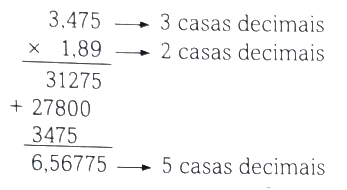
\includegraphics[width=1\linewidth]{6FMA57_imagens/imagem1}
	\noindent\textsubscript{---------------------------------------------------------------------}
    	\begin{enumerate}
    		\item Calcule:
    		\begin{enumerate}[a)]
    			\item 8,32 - 4,6 \\\\\\\\\\\\\\
    			\item 3,942 - 5,17 \\\\\\\\\\\\\\
    		\end{enumerate}
    		\item Em um parque há um brinquedo que precisa ser reformado. Para isso, serão confeccionadas duas escadas iguais, feitas com tubos de ferro, todos com o mesmo diâmetro. Considere a figura abaixo, onde estão indicadas as medidas das escadas:
    		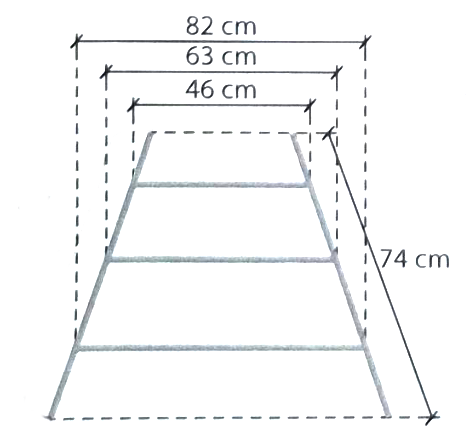
\includegraphics[width=1\linewidth]{6FMA57_imagens/imagem2}
    		Quantos metros de tubo são necessários para montar essas escadas? \\\\\\\\\\\\\\\\\\\\\\\\
    		\item Um marceneiro comprou uma dúzia de tábuas de 1,42 metro cada e 18 tábuas de 2,70 metros cada. O preço do metro da tábua é R\$ 0,94. Quanto o marceneiro pagou? \\\\\\\\\\\\\\\\\\\\\\\\\\\\\\\\
    		\item Mônica comprou uma coleção de 8 livros a R\$ 21,49 cada e pagou com duas notas de cem reais. Quanto recebeu de troco? \\\\\\\\\\\\\\\\\\\\\\\\\\\\
    		\item Maria comprou 8 canetas po R\$ 5,20 cada. Se ela pagou com uma nota de cinquenta reais, quanto Maria recebeu de troco? \\\\\\\\\\\\\\\\\\\\\\\\\\\\\\\\\\
    		\item Uma costureira comprou 12 rolos de 15,3 m de lã a R\$ 0,52 o metro e 9,15 m de seda a R\$ 2,33 o metro. As roupas feitas com esses materiais foram vendidas ao todo por R\$ 250,00. Qual foi o lucro da costureira? \\\\\\\\\\\\\\\\\\\\\\\\
    		\item O carro de Marcos faz 9 km com 1 litro de gasolina, que atualmente custa R\$ 3,92. Marcos anda por volta de 54 km por dia, todos os dias do mês. Quanto ele gasta de combustível em um mês, aproximadamente? Considere que em um mês há 30 dias. \\\\\\\\\\\\\\\\\\\\\\\\\\\\\\\\\\\\\\\\\\\\\\\\\\\\\\\\\\\\\\\\\\
    		\item Usando frações, explique por que a quantidade de casas decimais do produto de decimais é igual à soma das quantidades de casas dos fatores. \\\\\\\\\\\\\\\\\\\\\\\\
    	\end{enumerate}
    	$~$ \\ $~$ \\ $~$ \\ $~$ \\ $~$ \\ $~$ \\ $~$ \\ $~$ \\ $~$ \\ $~$ \\ $~$ \\ $~$ \\ $~$ \\ $~$ \\ $~$ \\ $~$ \\ $~$ \\ $~$ \\ $~$ \\ $~$ \\ $~$ \\ $~$ \\ $~$ \\ $~$
	\end{multicols}
\end{document}